% resume.tex
% vim:set ft=tex spell:

\documentclass[10pt,a4paper]{article}
\usepackage[a4paper,margin=0.70in]{geometry}
\usepackage{graphicx}
\usepackage[spanish]{babel}
\usepackage[utf8]{inputenc}
\usepackage{mdwlist}
\usepackage{textcomp}
\usepackage{tgpagella}
\pagestyle{empty}
\setlength{\tabcolsep}{0em}

% indentsection style, used for sections that aren't already in lists
% that need indentation to the level of all text in the document
\newenvironment{indentsection}[1]%
{\begin{list}{}%
	{\setlength{\leftmargin}{#1}}%
	\item[]%
}
{\end{list}}

% opposite of above; bump a section back toward the left margin
\newenvironment{unindentsection}[1]%
{\begin{list}{}%
	{\setlength{\leftmargin}{-0.5#1}}%
	\item[]%
}
{\end{list}}

% format two pieces of text, one left aligned and one right aligned
\newcommand{\headerrow}[2]
{\begin{tabular*}{\linewidth}{l@{\extracolsep{\fill}}r}
	#1 &
	#2 \\
\end{tabular*}}

% and the actual content starts here
\begin{document}

\begin{center}
{\LARGE \textbf{Mario Daniel Ruiz Saavedra}}

Carrera 26 \# 10 - 13\ \ 
\ \ Urbanización Country Club Villas\ \ \textbullet
\ \ Puerto Colombia, Atlántico, Colombia
\\
310 626 1218\ \ \textbullet
\ \ desiderantes93@gmail.com\ \ \textbullet \ \ https://github.com/desiderantes
\\
CC. 1082976380 \ \ \textbullet \ \ Nacido en Barranquilla, \ \ 1993-08-04


\vspace{0.4em}
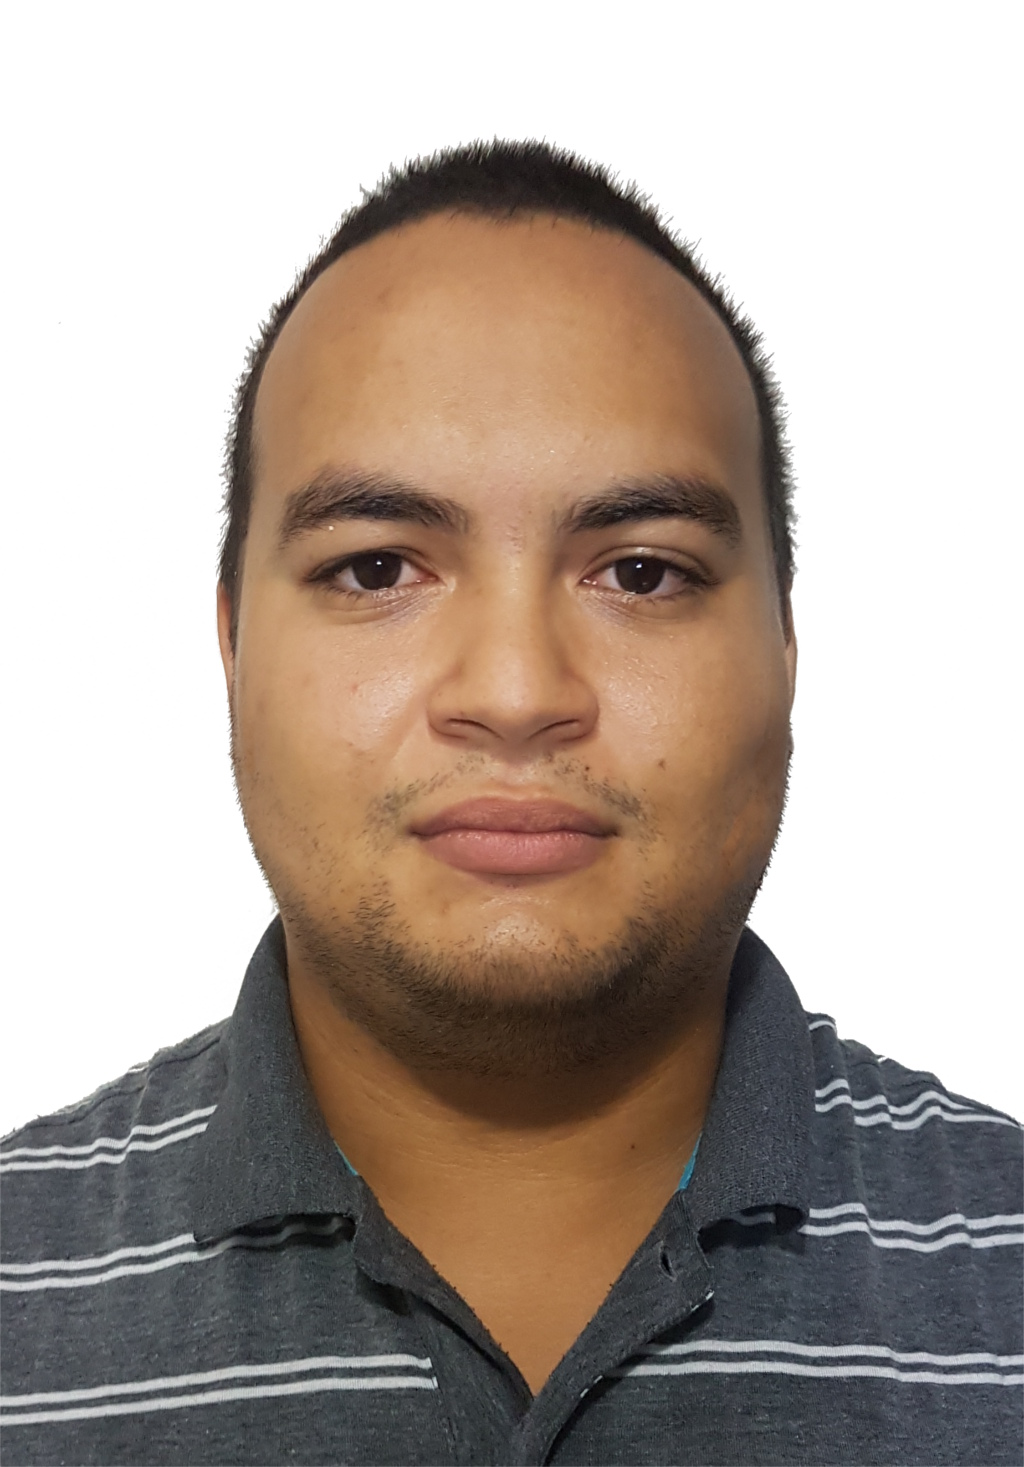
\includegraphics [width=6cm,height=6cm,keepaspectratio]{Foto.jpg}
\end{center}
\hrule
\vspace{-0.4em}
\subsection*{Experiencia}

\begin{itemize}
	\parskip=0.1em

	\item
	\headerrow
		{\textbf{Accendo S.A.S}}
		{\textbf{www.accendo.com.co}}
	\\
	\headerrow
		{\emph{Desarrollador Junior}}
		{\emph{julio de 2015 - septiembre de 2016}}
	\begin{itemize*}
		\item 
		\headerrow
		{\textbf{TerraInnova}}
		{\emph{julio de 2015 – octubre de 2015}}

		TerraInnova es un portal de contacto y gestión para productores y compradores de productos agrícolas. El desarrollo de aplicativo contó con un backend utilizando Java con Spring MVC, jOOQ, PostgreSQL, y el frontend con Thymeleaf, Bootstrap y jQuery. El portal corre sobre un sistema CentOS 7, y se usa AWS para la capa de datos.
		
		\item 
		\headerrow
		{\textbf{WColombia}}
		{\emph{octubre de 2015 – marzo de 2016}}
		Desarrollo de aplicativo web para control de inventario para empresa dedicada a la distribución de máquinas tragamonedas, teniendo en cuenta todos las variables que esta necesita y los impuestos asignados por el gobierno para este tipo de actividades. Esto se realizó con Spring Framework MVC, donde la persistencia de datos ocupó JPA, jOOQ y PostgreSQL. El frontend se desarrolló con Bootstrap 3 + jQuery.
		\item 
		\headerrow
		{\textbf{Crisálida}}
		{\emph{enero de 2016 – abril de 2016}}
		Crisálida es una iniciativa del gobierno para promover información relacionada con educación sexual, convivencia, y derechos de los niños y adolescentes. El portal desarrollado permite tomar encuestas, inscripción de estudiantes y actores del proyecto, alarmas de incidentes, y generación de reportes. El backend utiliza Spring Data, Spring MVC, Spring Boot, jOOQ, y PostgreSQL. El frontend se creó utilizando Javascript (JSX) con React, Redux para el manejo de información, y Bootstrap 3 para el diseño.
		\item 
		\headerrow
		{\textbf{Sushi2Home}}
		{\emph{mayo de 2016 – julio de 2016}}
		Sushi2Home es un servicio de sushi a domicilio, con presencia web y en redes sociales. El servicio consiste en un servidor en Ruby on Rails, con PostgreSQL como motor de base de datos y corriendo una plataforma Shoppe personalizada. En el lado del administrador, existe un cliente que administra los pedidos y se encarga de las impresiones y asignaciones de comandas y facturas. También presenta una interfaz web, tanto del lado del consumidor, escrita en VanillaJS, como del lado administrador, que es una versión modificada de la ofrecida por Shoppe. El cliente de escritorio fue desarrollado con C{$^\sharp$} y WPF.
		\item 
		\headerrow
		{\textbf{Trackvy}}
		{\emph{diciembre de 2015 – septiembre de 2016}}
		Trackvy es un sistema de manejo de Inventarios mediante sistemas RFID. Realicé la extensión del cliente del lector WindowsCE, la creación de un portal de lecturas en C{$^\sharp$} y SQLite, la creación de un cliente de escritorio para el etiquetado y movimiento de inventario con Spring Context, JavaFX y H2, y la remodelación de la Interfaz Web y API. Se pasó de Angular, D3.js y Typescript a HTML5, jQuery, Chartist.js, Bootstrap 3 y Thymeleaf. 
	\end{itemize*}

\end{itemize}

\begin{itemize}
	\parskip=0.1em
	
	\item
	\headerrow
	{\textbf{Nativapps S.A.S}}
	{\textbf{www.nativapps.com}}
	\\
	\headerrow
	{\emph{Desarrollador Java}}
	{\emph{febrero de 2017 -}}
	\begin{itemize*}
		\item 
		\headerrow
		{\textbf{OpenMDM}}
		{\emph{febrero de 2017 –}}
		
		OpenMDM es un sistema de administración de dispositivos móviles. Permite llevar registro de la ubicación, estado, y conexión de los dispositivos de forma remota. También incluye un módulo de acceso remoto vía navegador, y un sistema de ejecución de comandos. El backend está escrito con MySQL, Java 8, jOOQ, Spring Framework, ActiveMQ, y Swagger para la documentación de la API.
		\end{itemize*}
	
\end{itemize}

\hrule
\vspace{-0.4em}
\subsection*{Certificaciones}

\begin{itemize}
	\parskip=0.1em

	\item 
	\headerrow
		{\textbf{Programación de páginas Web con HTML y JavaScript}}
		{\textbf{SENA}}
	\\
	\headerrow
		{\emph{Licencia SGCV20102985332}}
		{\emph{diciembre de 2010}}
	\begin{itemize*}
		\item Desarrollo de páginas web con HTML, ECMAScript 5 y CSS 3
	\end{itemize*}

\end{itemize}

\hrule
\vspace{-0.4em}
\subsection*{Educación}

\begin{itemize}
	\parskip=0.1em

	\item 
	\headerrow
		{\textbf{Colegio Gimnasio Bolivariano}}
		{\textbf{Santa Marta, Colombia}}
	\\
	\headerrow
		{\emph{Bachiller con énfasis en ciencias naturales}}
		{\emph{1997 - 2009}}

	\item 
	\headerrow
	{\textbf{Universidad del Norte}}
	{\textbf{Barranquilla, Colombia}}
	\\
	\headerrow
	{\emph{Ingeniería de Sistemas y Computación}}
	{\emph{2012 - (en pausa)}}
	\begin{itemize*}
		\item Deseo hacer énfasis en el desarrollo de componenetes de sistema a bajo nivel, de preferencia en sistemas UNIX-like o UNIX-Next (como Plan9)
		\item Mis intereses se enfocan a escribir subsistemas útiles 
	\end{itemize*}
	

\end{itemize}


\hrule
\vspace{-0.4em}
\subsection*{Habilidades de profesión}

\begin{indentsection}{\parindent}
\hyphenpenalty=1000
\begin{description*}
	\item[Lenguajes manejados:]
	C, Vala, Java, JavaScript, \LaTeX, HTML, C{$^\sharp$}, JSX, SQL
	\item[Frameworks y Librerías manejados:]
	Spring (Boot, MVC, Data, Cloud, JPA), React, Redux, jQuery, Bootstrap 3, Hibernate, Thymeleaf, jOOQ, JavaFX, Glade, WPF.
	\item[Herramientas manejadas:]
	GNU/Linux, Git, Vagrant, IntelliJ IDEA, nano, KVM, GIMP, Inkscape, LibreOffice Writer
	\item[Contribuciones de Software Libre:]
	ValaVerbalExpressions (autor), SDL2 Bindngs for Vala (coautor), Stew build system (mantenedor)
\end{description*}
\end{indentsection}
\hrule
\vspace{-0.4em}
\subsection*{Referencias}
\begin{indentsection}{\parindent}
\hyphenpenalty=1000
\begin{description*}
	\item[Familiares:]
	
	\begin{itemize*}
		\
		\item
		\item Carmen Nidia Saavedra Ruz - Abogada de Familia - 3103631187
		\item Hernan Darío Ruiz Soler - Ingeniero de Sistemas - 3013437656
		\item Ruben Darío Ruiz Becerra - Ingeniero Mecánico - 3103574030
	\end{itemize*}

	\item[Personales:]
	
	\begin{itemize*}
		\
		\item
		\item Stefanny Espinosa - Ingeniera Electrónica -  3145951482
		\item Carlos Arbey Bolaños Duarte - Ingeniero Electrónico -  3005307422
		\item Jhon Jairo Ruiz Soler - Antropólogo - 3002426851
	\end{itemize*}
\end{description*}
\end{indentsection}

\end{document}
